\documentclass[12pt,a4paper]{article}
\usepackage[utf8]{inputenc}
\usepackage[margin=1in]{geometry}
\usepackage{graphicx}
\usepackage{float}
\usepackage{amsmath}
\usepackage{listings}
\usepackage{xcolor}
\usepackage{algorithm}
\usepackage{algpseudocode}
\usepackage{enumitem}

% Code listing style
\lstset{
    language=C++,
    basicstyle=\ttfamily\footnotesize,
    keywordstyle=\color{blue},
    commentstyle=\color{green},
    stringstyle=\color{red},
    numbers=left,
    numberstyle=\tiny,
    frame=single,
    breaklines=true
}

\begin{document}

% Front Page
\begin{titlepage}
  \centering
  \vspace*{3cm}

  {\Huge\bfseries CSE 406 – Lab Report 4: Non-Preemptive Priority Scheduling Algorithm \par}
  \vspace{2.5cm}

  \noindent
  \begin{minipage}[t]{0.48\textwidth}
    {\large\bfseries Submitted By:}\\[0.5em]
    \Large
    Sharif Md. Yousuf \\
    ID: 22101128 \\
    Section: C-2 \\
    4th Year, 1st Semester \\
    Spring 2025
  \end{minipage}
  \hfill
  \begin{minipage}[t]{0.48\textwidth}
    {\large\bfseries Submitted To:}\\[0.5em]
    \Large
    Atia Rahman Orthi \\
    Lecturer \\
    Department of Computer Science \& Engineering \\
    University of Asia Pacific
  \end{minipage}

  \vfill

  {\Large\bfseries Date of Submission:} \\[0.5em]
  {\LARGE\bfseries 16 August, 2025 (Saturday)}

  \vspace*{2cm}
\end{titlepage}

\section{Problem Statement}
We are to implement a non-preemptive Priority CPU scheduling algorithm. Each process is defined by: Process ID, Arrival Time (AT), Burst Time (BT), and Priority (PR) where a lower numerical value indicates a higher scheduling priority. The scheduler must always select, among the processes that have arrived and not yet completed, the process with the highest priority (lowest PR). Ties are broken first by earliest arrival time and then lexicographically by process ID. The program must compute Completion Time (CT), Turnaround Time (TAT = CT - AT) and Waiting Time (WT = TAT - BT) for every process and report average TAT and WT. Idle CPU periods must be handled when no process has arrived at the current time.

\subsection*{Input}
\begin{itemize}
  \item First line: an integer $n$ ($n>0$) denoting the number of processes.
  \item Next $n$ lines: each line contains four tokens: \texttt{PID AT BT PR}
  \begin{itemize}
    \item \texttt{PID}: a string without spaces (e.g., P1, A, T3)
    \item \texttt{AT}: non-negative integer arrival time
    \item \texttt{BT}: positive integer CPU burst time
    \item \texttt{PR}: non-negative integer priority (smaller value = higher priority)
  \end{itemize}
\end{itemize}

Example:
\begin{verbatim}
5
P1 0 4 2
P2 1 3 1
P3 2 2 3
P4 4 4 2
P5 5 3 1
\end{verbatim}

\subsection*{Output}
\begin{itemize}
  \item A header line listing the column titles, e.g.:
\begin{verbatim}
PID AT BT PR CT TAT WT
\end{verbatim}
  \item One line per process in the internal (sorted/executed) order with computed metrics.
  \item Two summary lines giving average Turn Around Time and average Waiting Time to two decimal places.
\end{itemize}

Example (for the sample above --- values depend on scheduling order):
\begin{verbatim}
PID	AT	BT	PR	CT	TAT	WT
P1	0	4	2	4	4	0
P2	1	3	1	8	7	4
P3	2	2	3	10	8	6
P4	4	4	2	14	10	6
P5	5	3	1	17	12	9

Average Turn Around Time: 8.20
Average Waiting Time: 5.00
\end{verbatim}

\section{Objective}
In this lab we aimed to:
\begin{itemize}
    \item Understand the working principle of non-preemptive priority-based scheduling
    \item Implement deterministic tie-breaking for reproducible ordering
    \item Correctly manage CPU idle intervals by advancing to the next arrival
    \item Compute per-process and average performance metrics (CT, TAT, WT)
    \item Analyze fairness, starvation risk, and efficiency characteristics
\end{itemize}

\section{Source Code Screenshot}
If included, add a screenshot named \texttt{code.png} in this folder for compilation. (Placeholder omitted here.)

\begin{figure}[H]
  \centering
  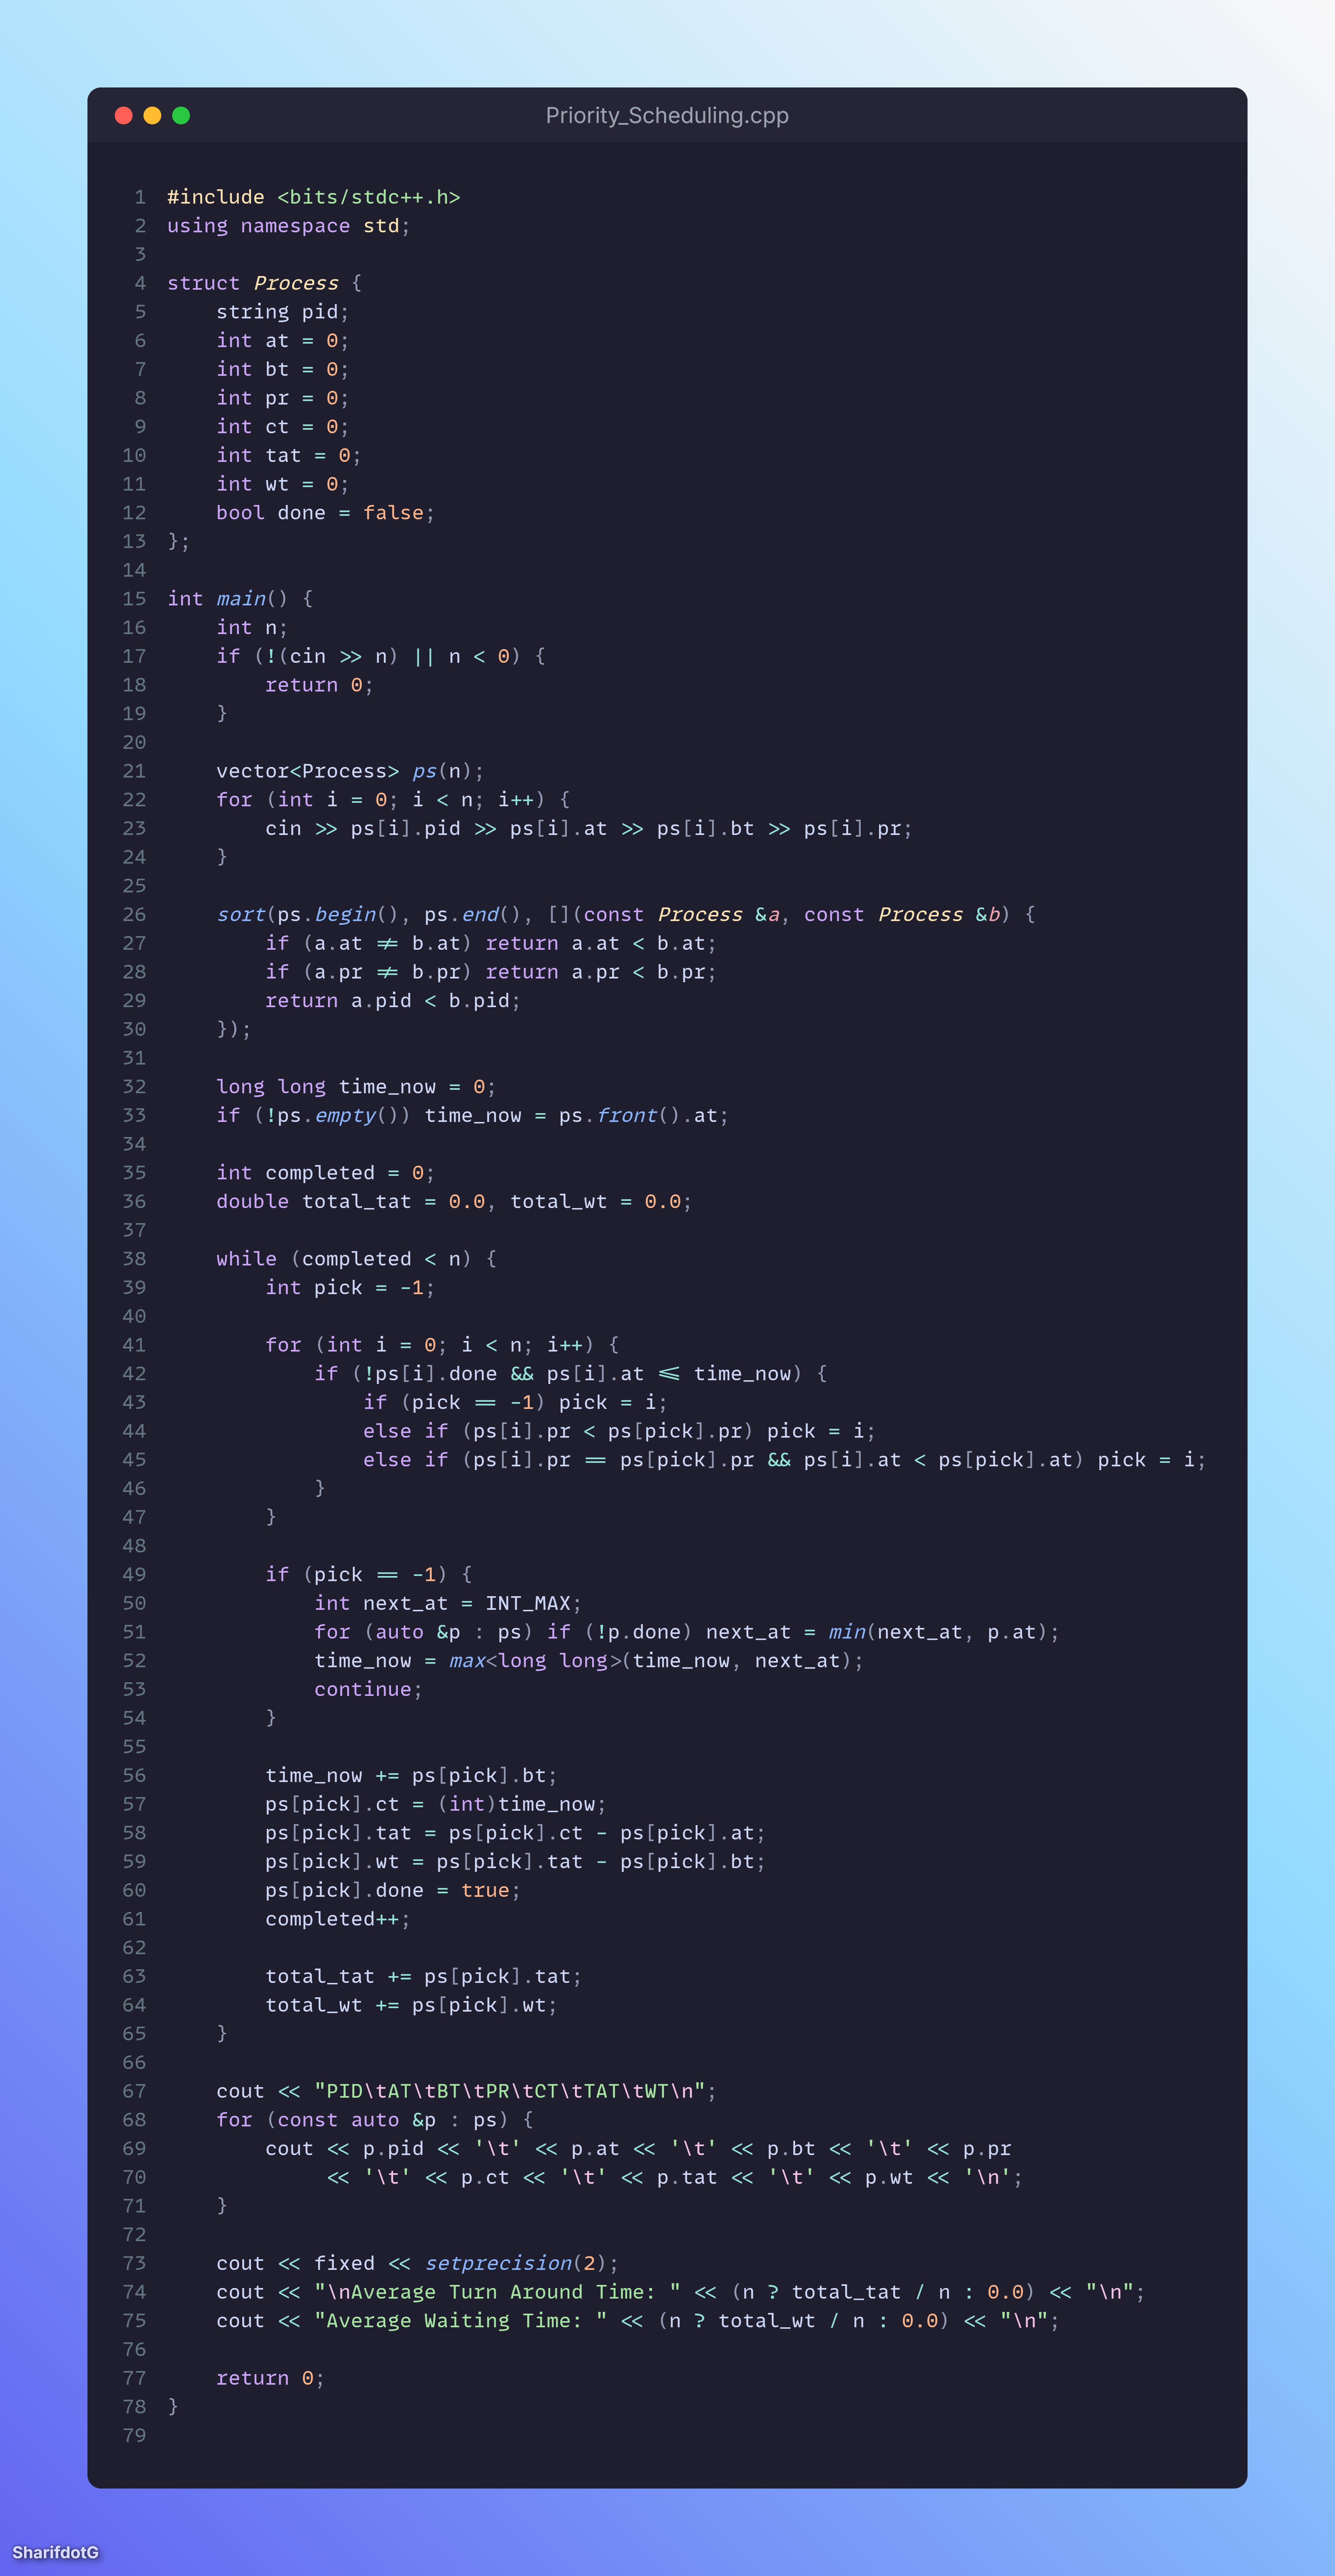
\includegraphics[width=0.85\textwidth]{Code.png}
  \caption{Priority Scheduling Source Code}
\end{figure}

\section{Output Screenshot}
\begin{figure}[H]
  \centering
  \includegraphics[width=0.85\textwidth]{Screenshot 2025-08-16 234650.png}
  \caption{Program Output}
\end{figure}

\section{Discussion}
Priority scheduling favors higher-priority (numerically smaller) processes, improving response time for critical tasks. However, non-preemptive behavior means once a lower-priority but long job starts, an immediately arriving higher-priority job must wait until completion, increasing potential latency.

\textbf{Starvation Risk:} If high-priority processes continue to arrive, very low-priority jobs could experience indefinite postponement. Aging (gradually decreasing priority values over waiting time) is a common mitigation not implemented here.

\textbf{Determinism:} Explicit tie-breaking ensures reproducibility which aids debugging and grading.

\textbf{Idle Handling:} Jumping the clock directly to the next arrival prevents unnecessary iteration simulating empty time units.

Compared to FCFS, average waiting time can be lower when priorities correlate with short tasks. Compared to SJF, priority may not always reflect burst length, so optimal waiting time minimization is not guaranteed. Unlike Round Robin, this algorithm is not time-sharing and can produce larger response times for late-arriving urgent tasks unless preemption or aging is added.

\section{Conclusion}
The non-preemptive priority scheduling implementation correctly computes essential metrics and demonstrates trade-offs between responsiveness for important tasks and fairness for low-priority workloads. Extensions such as preemptive priority scheduling and aging would address starvation and improve responsiveness for newly arrived critical tasks.

\end{document}
